\documentclass[12pt,a4paper]{article}
\usepackage{graphicx}
\usepackage{amsmath}
\usepackage{bm}
\usepackage{interval}
\begin{document}

\section*{Problem 5}
ChatGPT says:
\newline
A notable application of active learning in machine learning is in data labeling for supervised learning tasks.
\newline
Example: Data Labeling with Active Learning
\newline
In this scenario, an active learning algorithm selectively queries a human annotator to label the most informative data points from a large, unlabeled dataset. Here is how it works:
\begin{enumerate}
    \item Initial Model Training: A preliminary model is trained on a small labeled dataset.
    \item Uncertainty Sampling:The model identifies which unlabeled data points it is least confident about (e.g. those near the decision boundary). 
    \item Querying for Labels: The model then queries the human annotator to label these uncertain data points, rather than labeling the entire dataset.
    \item Model Improvement: The newly labeled data is added to the training set, and the model is retrained to improve its accuracy.
    \item Iterative Process: This process is repeated, with the model continuously refining its predictions and focusing on the most challenging samples.
\end{enumerate}
By using active learning in this way, the model can achieve high performance with significantly less labeled data, making it especially useful in situations where labeling is costly or time-consuming.
\newline
\hspace*{\fill}
\newline
\textbf{My arguement:}
\newline
Active learning focus on question asking. The example supplied by ChatGPT is good.
It is a standard application of active learning. Since the data we want to label would be a large amount,
we cannot label them manually. We can first label a few numbers of the data to let machine learn, 
then let machine help us to label the data which we have not labeled. In the labeling process, the agent will ask us
the data it has less confidence. From the asking, the agent can label the data more correctly.

\newpage
\section*{Problem 6}
ChatGPT says:
\newline
Machine learning can be utilized to analyze patterns in seismic data and potentially improve earthquake prediction efforts, though it's important to note that accurately predicting earthquakes remains a complex challenge.
\newline
\begin{enumerate}
    \item How Machine Learning Can Help: Seismic Data Analysis: Machine learning algorithms can analyze vast amounts of seismic data from sensors and historical earthquake records to identify patterns and anomalies that may precede seismic events.
    \item Feature Extraction: Algorithms can extract relevant features from raw seismic signals, such as frequency patterns, amplitude changes, or other geophysical characteristics that might indicate an impending quake.
    \item Classification Models: Supervised learning models can be trained to classify seismic events, distinguishing between typical seismic noise and potentially significant tremors.
    \item Anomaly Detection: Unsupervised learning techniques can help identify unusual patterns in seismic data that may signal an increased risk of an earthquake.
    \item Real-Time Monitoring: Machine learning can enhance real-time monitoring systems by providing quicker assessments of seismic activity and improving alert systems for potential earthquakes.    
\end{enumerate}
Limitations:
While machine learning offers valuable tools for analyzing seismic data, accurately predicting the exact time, location, and magnitude of earthquakes is still beyond current capabilities.
Earthquakes are influenced by complex geological processes that are not fully understood, making precise predictions difficult.
However, machine learning can contribute to better understanding seismic risks and enhancing preparedness.
\newline
\hspace*{\fill}
\newline
\textbf{My arguement:}
\newline
The answer from ChatGPT is very useful. Since we have not analyzed the reason why earthquake occurs completely,
we can only recognize earthquake by the features we have already known. Machine learning is a great tool to help us
analyze the data we collected from the happened earthquake. This question is the question we want to find x from getting y.
By using machine learning, we can find the relativity between any features we've collected and the earthquake.
ChatGPT gives us a great and detailed.

\newpage
\section*{Problem 10}
We can observe that the distribution of the update times of the weight $\bm{w}$ is concentrated around 100.
Most of them are in the interval $\interval{95}{105}$, which is about $\frac{N}{2}$.
By the figure 1, we can find out that the update times is about half of the numbers of the data.
\begin{figure}[hbp]
    \centering
    \begin{minipage}{0.48\linewidth}
        \centering
        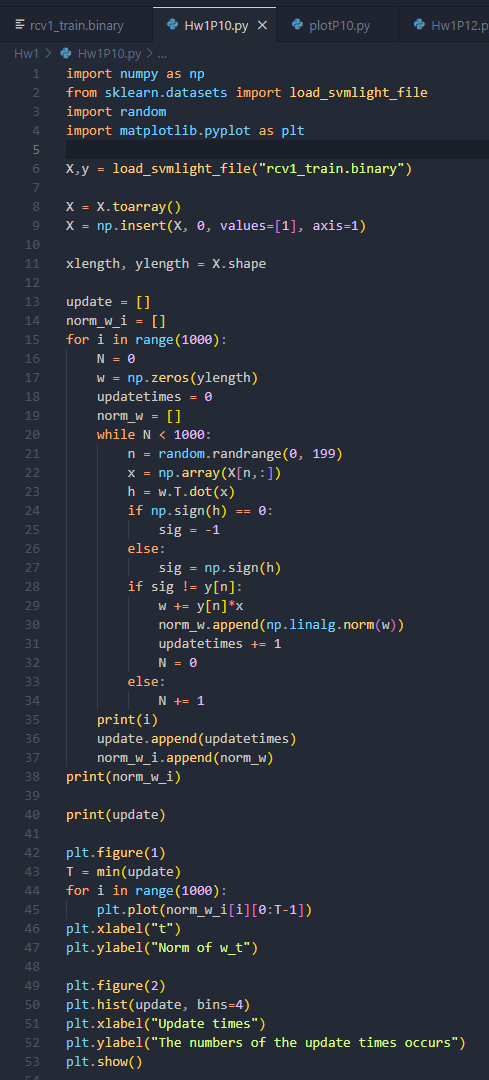
\includegraphics[width = \linewidth]{Hw1P10 snapshot.png}
        \caption{snapshot}
    \end{minipage}\hfil
    \begin{minipage}{0.48\linewidth}
        \centering
        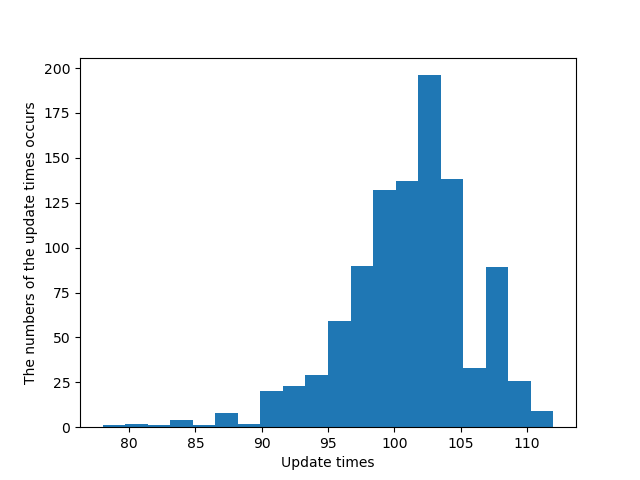
\includegraphics[width = \linewidth]{Hw1P10.png}
        \caption{historgram}
    \end{minipage}\hfil
\end{figure}
\newpage
\section*{Problem 11}    

\begin{figure}[hbp]
    \centering
    \begin{minipage}{0.48\linewidth}
        \centering
        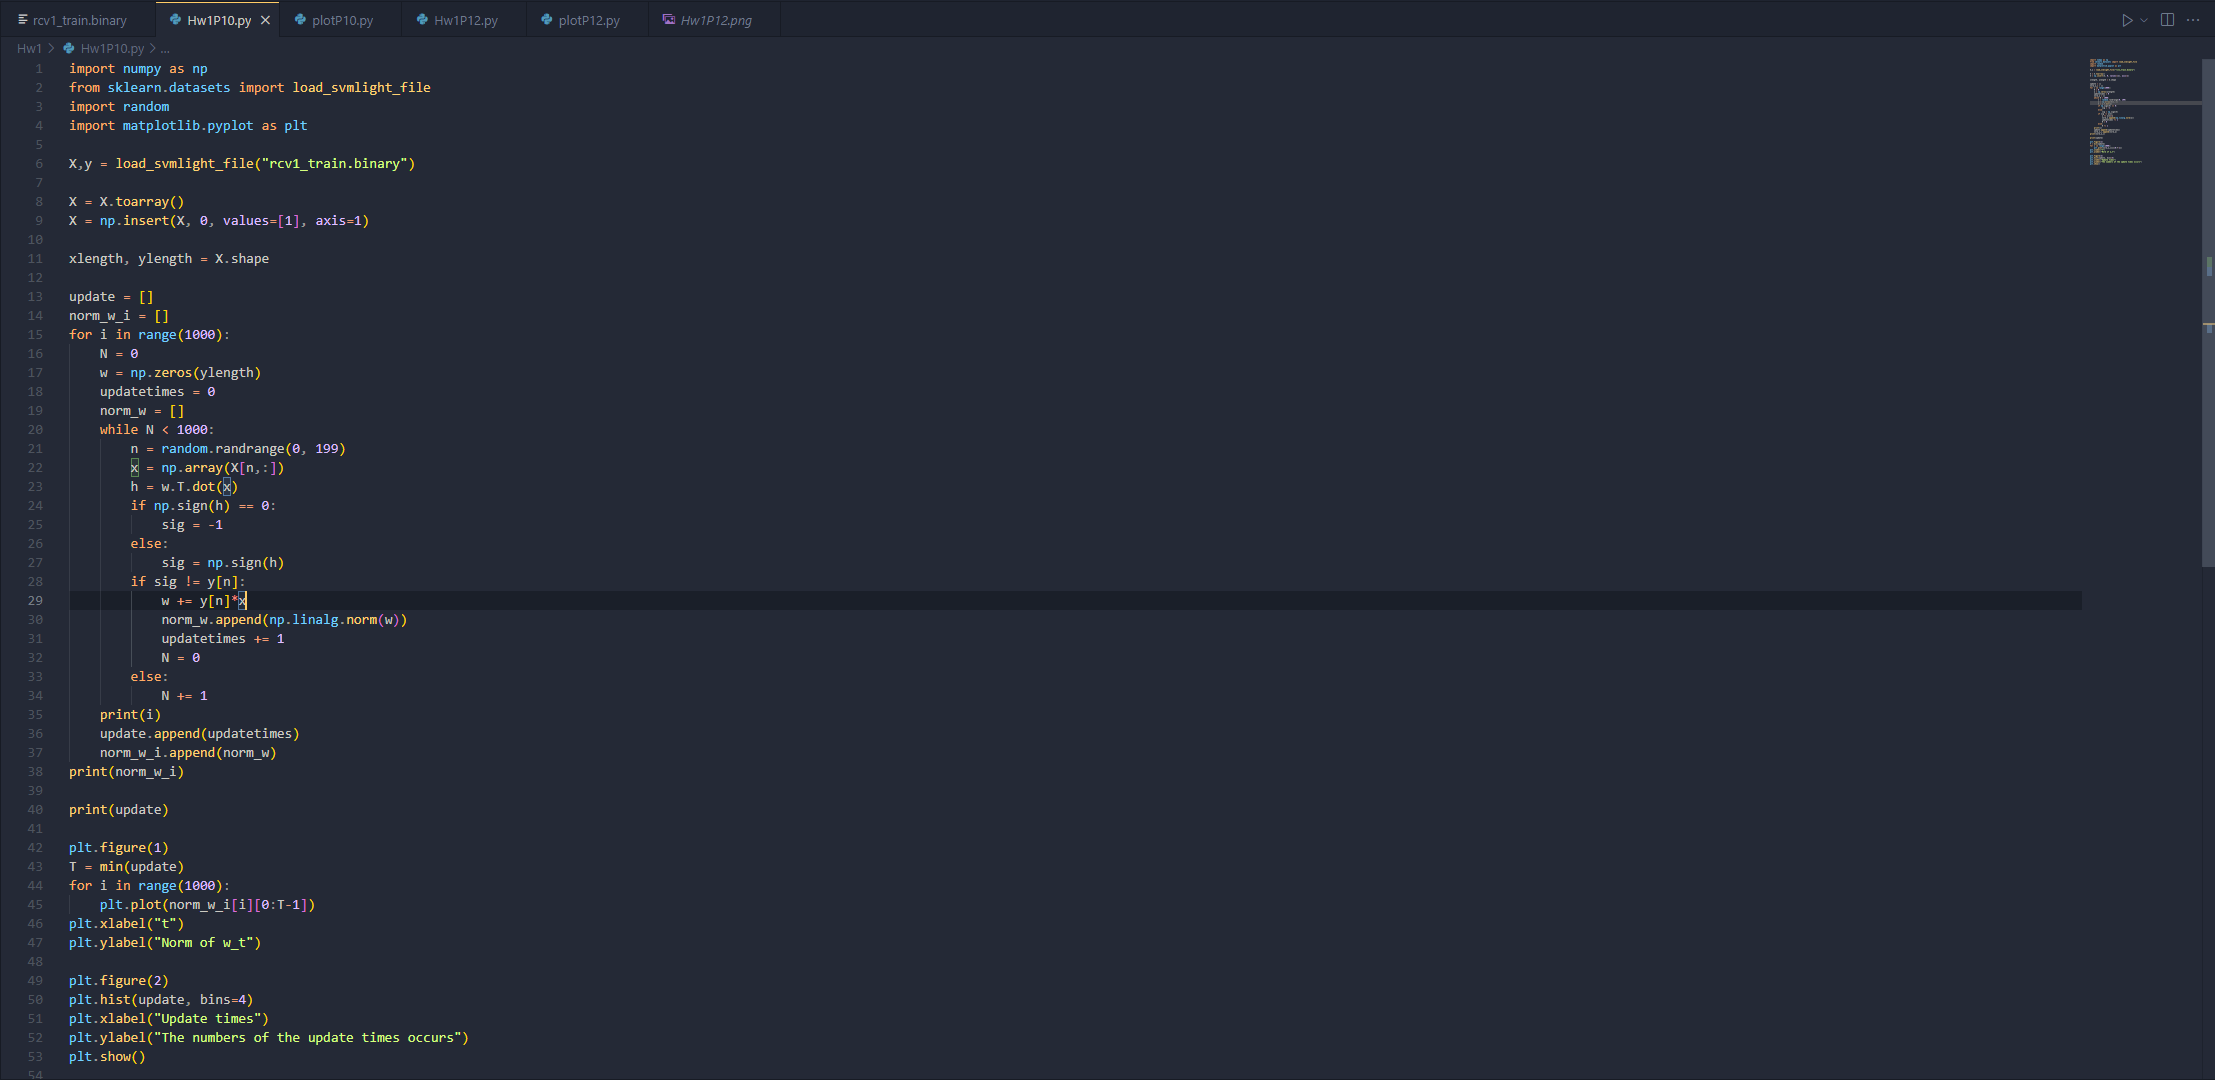
\includegraphics[width = \linewidth]{Hw1P11 snapshot.png}
        \caption{snapshot}
    \end{minipage}\hfil
    \begin{minipage}{0.48\linewidth}
        \centering
        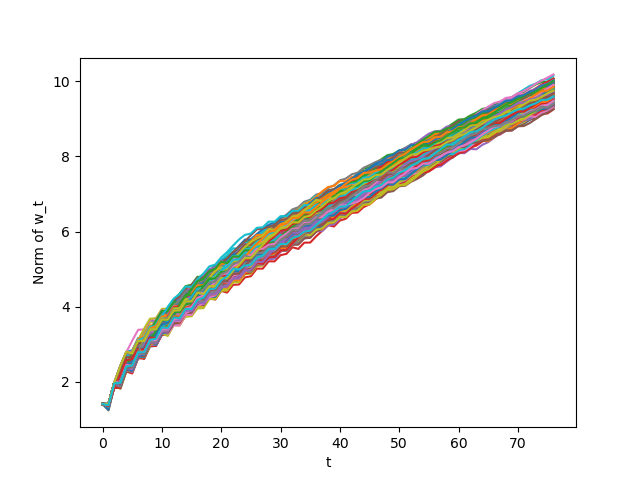
\includegraphics[width = \linewidth]{Hw1P11.png}
        \caption{plot}
    \end{minipage}\hfil
\end{figure}

\newpage
\section*{Problem 12}    
For the P12, we update $n(t)$ only when $\bm{w}_{t}$ does not change. 
Compare with Figure 2 we can observe that most of the update times are still in $\interval{95}{105}$.
But it looks more concentrated then the histogram in P10. That is, the update times are more stable than P10.   
\begin{figure}[hbp]
    \centering
    \begin{minipage}{0.48\linewidth}
        \centering
        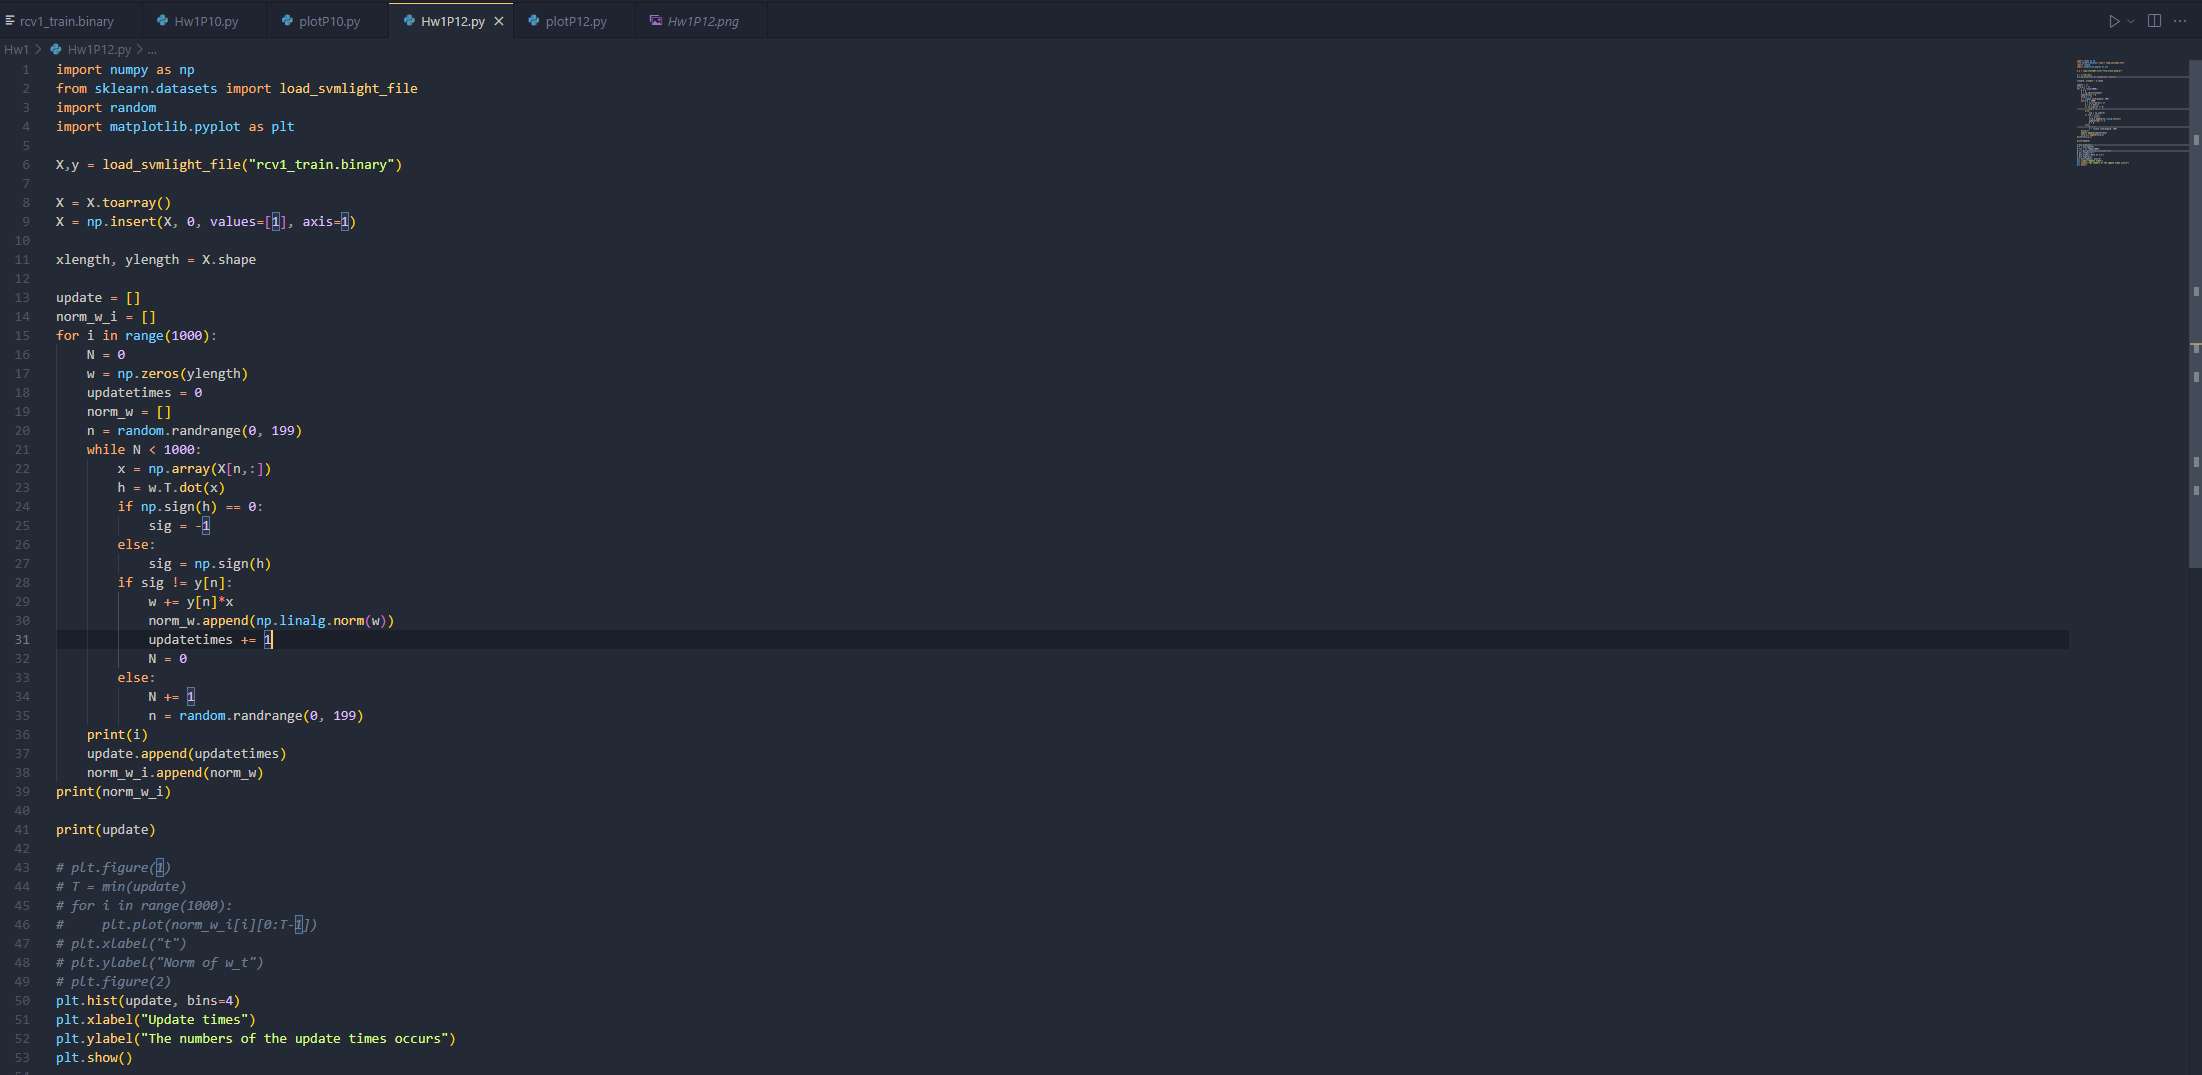
\includegraphics[width = \linewidth]{Hw1P12 snapshot.png}
        \caption{snapshot}
    \end{minipage}\hfil
    \begin{minipage}{0.48\linewidth}
        \centering
        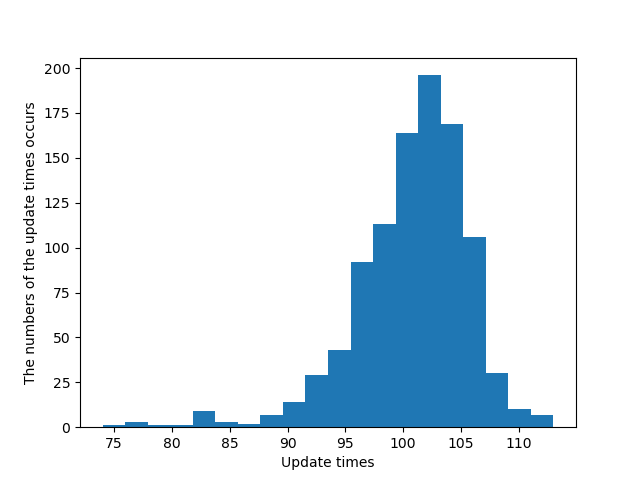
\includegraphics[width = \linewidth]{Hw1P12.png}
        \caption{historgram}
    \end{minipage}\hfil
\end{figure}
\end{document}
